\section{Etude des solutions d'architecture}

\subsection{Scénario d'Urbanisation du SI}

Afin de répondre aux besoins exprimés par le client, nous proposons une solution de déploiement basée sur une architecture d'intégration d'application, autrement dit EAI. 
En effet, l'un des principaux constats effectués après l'analyse de l'existant de l'entreprise est que cette dernière possède bien un SI performant et adapté à ses besoins, du moins dans la partie opérationelle... En ce qui concerne le coté analytique cela se révèle un peu moins proche de la réalité, ceci est notamment lié à la vétusté des équipements en activité.

\subsubsection{Lignes directrices du projet}

Nous avons donc décidé de proposer une architecture typée par site. Plusieurs clés pour cette architecture :\\

\begin{itemize}
\item Réplication des services par site, permettant un fonctionnement assuré en mode dégradé du SI
\item Typage du SI des différents sites relativement aux services utilisés sur ces derniers
\item Intégration des applications opérationelles existantes dans d'une architecture typée EAI
\item Déploiement d'une orchestration de service SOA
\item Refonte du segment data Warehouse et business intelligence, avec des problématiques de qualité\\
\end{itemize}

Afin d'optimiser le fonctionnement de votre entreprise, nous prévoyons d'intégrer un système d'orchestration de services SOA, basé sur la modélisation de vos activités sous forme de processus industriels, formant votre chaine de valeur.\\
Chaque entité de l'entreprise possède sa propre base de donnée opérationelle, servant d'entrepot de données local à chaque site. Chaque application opérationelle déployée est synchronisée par un connecteur ESB développé spécifiquement, ainsi chaque site possède son propre sous enssemble de data Warehouse, qui est ensuite synchronisé et intégré au data warehouse principal, hébergé à la DSI du site central. Ainsi, si le WAN de l'entreprise est indisponible, le mode de fonctionnement dégradé permet d'éviter l'arrêt de vos activités.\\
Notons aussi, le déploiement d'un système de Master Data Management pour la qualité globale des données hébergées. Ce système à la pointe de la technologie des systèmes d'information permet d'assurer une gestion de la qualité du premier ordre dans votre système d'information.\\
Enfin, nous prévoyons une refonte complète de la partie analytique de votre entreprise, afin d'y intégrer un applicatif de BI de dernière génération pour le suivi de vos activités, et des outils de dataMining pour effectuer de l'analyse prédictive.\\

Ainsi, comme nous allons le découvrir, cet architecture permettant de mettre  à profit un existant déjà performant et adapté à vos besoins, permet d'envisager à nouveau un système évolutif, doté des dernières technologies en terme de qualité de données et de business intelligence, permettant un pilotage de vos activités le plus précis posssible.\\

\subsubsection{Architecture \& Service hébergés}

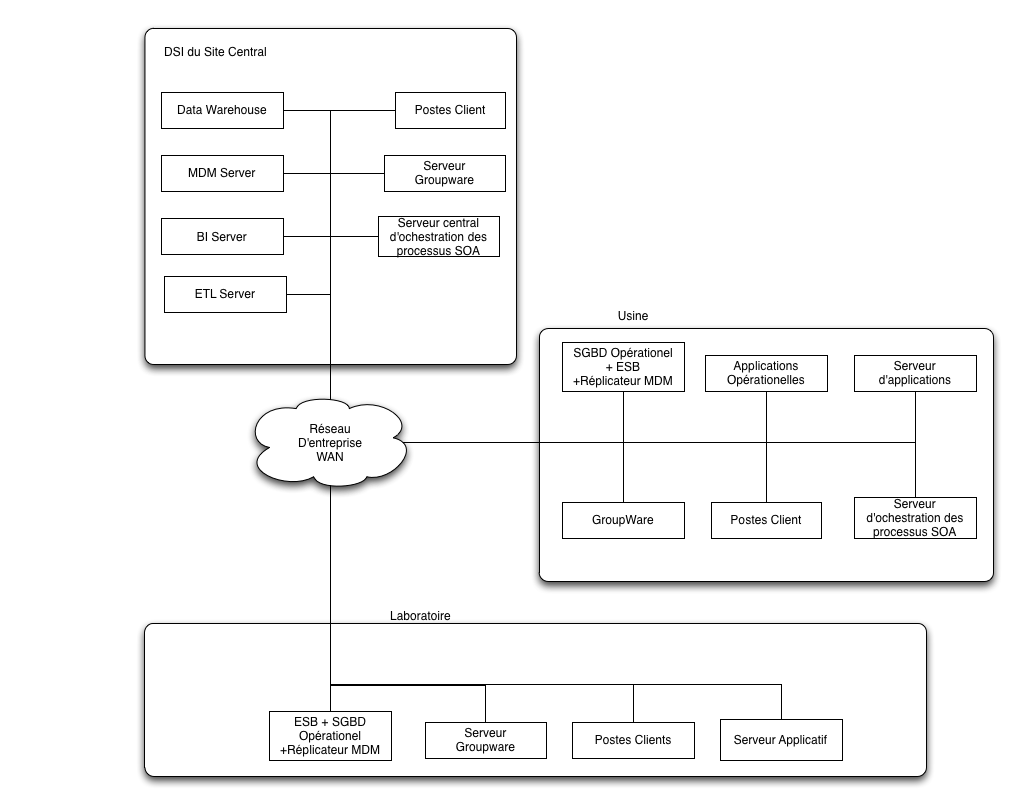
\includegraphics[scale=0.2]{DiagrameSOAPdc4.png}

\subsubsection{Infrastructure de support technique}
Afin de simplifier l'exploitation, nous proposons que l'architecture logicielle proposée soit supportée par une achitecture basée sur des machines virtuelles, limitant grandement le nombre de machines de type serveur à déployer.
Les systèmes virtuels sont facilement manipulables et peuvent être restaurés simplement en cas de défaut de machines.\\
Bien entendu les infrastructures de transport, passives et actives sont à prévoir sur les différents sites, si elles n'existent pas déjà.

\subsubsection{Architecture pour le site central}

Le site central est dans ce scenario le centre névralgique du système d'information de l'entreprise. Les services hébergés sont les suivants :\\

\begin{itemize}
\item Main dataWarehouse : Principal entrepôt de données de l'entreprise, c'est lui qui constitue la base de travail pour les application de business intelligence.
\item MDM Server :  Serveur de Master data Management, en charge de la génération, du maintien, et de l'exposition aux applications utilisatrices de la base d'exploitation de données de références.
\item BI Server : Hébergment des principaux services de business intelligence, système de reporting, générateurs de tableaux de bords et applicatif dédié au DataMining.
\item ETL Server : En charge de l'alimentation du dataWarehouse, assure la synchronisation des données entre les différents SGBD opérationnels déployés sur les différents sites, et la synchro réciproque entre le datawarehouse et le système de master data management.
\item Serveur central d'orchestration SOA : Serveur en charge de l'orchestration des principaux processus et méta-processus de l'entreprise, il pilote les services d'orchestration déployés dans chaque site.
\item Serveur Groupware, dédié au travail collaboratif.
\end{itemize}

La totalité des postes présents sont réutilisés, moyennant éventuellement un redéploiement de ces derniers. De plus, la création d'une DSI implique l'équipement des effectifs de ce service.

\subsubsection{Achitecture pour laboratoire \& Usine}

Chaque entité de l'entreprise possède son propre SI autonome, permettant un fonctionnement de l'entreprise en mode dégradé. ( Site principal in joignable...)
Toute la finesse de la solution se trouve au niveau de la décentralisation des bases de données opérationnelles, qui sont par la suite agrégées au niveau du site principal \\
Pour parvenir  à cela, nous dotons le serveur de BDD de trois fonctionnalités principales.
\begin{itemize}
\item SGBD : Serveur de BDD classique, hébergeant toutes les données opérationnelles nécessaires au fonctionnement du site.
\item ESB : Système de synchronisation et de communication entre le serveur de BDD et les application opérationelles utilisatrices.
\item MDM replication Server :  Serveur de rapatriement et de stockage des données de références du SI, permettant l'exploitation des données de références nécessaire au fonctionnement des application opérationnelles.
\end{itemize}

Ensuite, les services proposés sont bien évidemment adaptés aux besoins des différents sites. Notons tout de même la présence d'un serveur d'orchestration SOA déporté pour controller les processus de fonctionnement des sites, très utile pour les usines de fabrication notamment, où l'avantage d'avoir une maitrise de l'activité par processus n'est plus à démontrer.

\subsubsection{Nouveaux services envisagés}

L'architecture proposée possède donc l'avantage avant tout de mettre en place une infrastructure évolutive, ou le développement et l'intégration de nouveaux services opérationnels destinés à  couvrir vos objectifs pour le système d'information.

\begin{itemize}
\item SSO / Ldap / CAS : Nous prévoyons la mise en place d'un système de centralisation des identités dans le SI, afin d'en augmenter la sécurité et l'extensibilité, notamment via l'intégration aux fournisseurs.
\end{itemize}

\subsection{Robustesse et tolérance aux incidents}

Compte tenu de l'architecture détaillée auparavant, nous avons réussi à limiter sur de nombreux aspects les risques pour le système d'information.\\

\subsubsection{Mode dégradé}

Du fait de son architecture hautement décentralisée et des mécanismes de synchronisation issues des dernières technologies en date, le système d'information de chaque site reste opérationnel même si la liaison entre le site central et les sites distant n'est plus opérationnel. De plus, la cohérence des données n'est en aucun cas remise en question les outils d'EAI, ESB et autres Data Management sont la pour assurer le tout !

\subsubsection{Réplication Géographique}
Autre point positif, les données sont automatiquement répliquées entre les différents sites et le site central, chaque site pouvant avoir besoin des données opérationnelles d'un autre site.\\
Ainsi, en cas de sinistre important sur l'un des sites, les risques de perte de données seront minimisés car ces dernières sont automatiquement répliquées sur les autres sites et le serveur central.

\subsection{Impact organisationnel}

Deux points de vue en réponse à cette question\\
\begin{enumerate}
\item Internalisation des compétences : création d'une DSI, et embauche des personels ayant la compétence de développement des connecteurs d'intégration, de déploiement et de maintenance de l'installation par étape. Ce choix ayant un coût fixe, il permet d'éviter de créer un lien de dépendance entre vous et une entreprise prestataire de services en informatique.
\item Externalisation de la maintenance informatique : Il s'agit d'évaluer et de vérifier si votre actuel prestataire possède les compétences nécessaires, pour effectuer ce type de démarche, qui s'avère relativement difficile d'externaliser au final, du fait de la phase de développement spécifique, nécessitant un temps relativement long entre la première recette et la phase de stabilité opérationelle.
\end{enumerate}

\subsection{Conclusion}


\subsection{Scénario de déploiement d'un ERP}
Le scénario que nous allons décrire ci dessous est une directive à prendre pour l'entreprise pour les 5 années à venir. Nous proposons à l'entreprise d'intégrer un ERP est plus particulièrement des modules adaptés à ces différents objectifs d'amélioration. 
\subsubsection{Présentation de la solution}
Cette solution consiste à intégrer au système existant un système d'ERP pour répondre aux besoins B2B de l'entreprise. Il propose des applications spécialisées pour la gestion des laboratoires (LIMS), de la relation client (CRM), de la maintenance (GMAO). Actuellement l'entreprise possède un SI fonctionnel et performant c'est pourquoi il n'est pas nécessaire de le modifier cependant il est intéressant pour l'entreprise de rajouter des fonctionnalités de gestion de certain processus. L'entreprise est composée d'un laboratoire central, structure contenant des données confidentielles, pour le moment sa gestion est similaire aux autres structures : usines, sièges et service central de maintenance. La solution que nous présentons dans ce scénario s'adapte parfaitement à l'entreprise en proposant un module dédié à la gestion du laboratoire, mais également aux autres besoins de l'entreprise : outils de pilotage, processus dédié au B2B.   
\paragraph{Architecture Applicative}
Voici une représentation des domaines qui seront gérer par le scénario que nous proposons de mettre en place :
\begin{figure}[H]
\begin{center}
 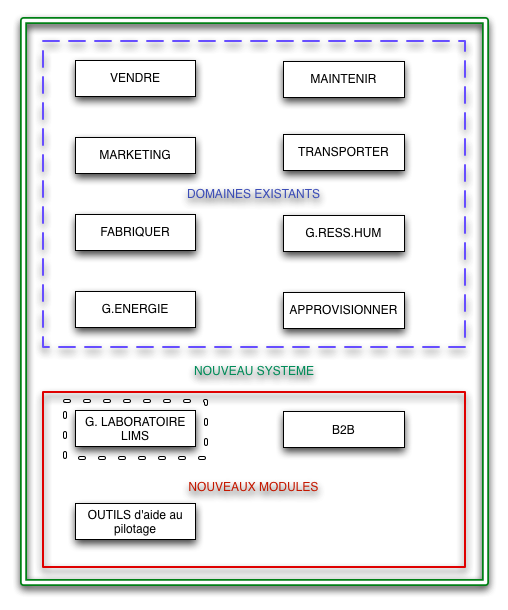
\includegraphics[scale=0.5]{ERPsolution.png}
  \caption{Nouveau système}
\end{center}  
\end{figure}

Nous proposons d'intégrer aux domaines existants : vendre, marketing, approvisionner, ...  des modules spécifiques dédiés à la gestion du laboratoire, au B2B et aux outils de pilotage. \\
Le module dédié à la gestion du laboratoire sera spécifique à l'entreprise alors que les modules de B2B et outils de pilotage seront à acheter. 

\paragraph{Architecture Logicielle}
Cette solution ne nécessite pas de logiciel mais d'héberger un soft sur un serveur. Chaque poste aura accès aux systèmes via un site internet. Il n'y a donc pas d'installation particulière à faire au niveau des sites.
\paragraph{Architecture matérielle}
Une base de donnée unique répliquée sur chaque sites sera installée au niveau d'EDS. Chaque site aura donc accès à une base de donnée en locale qui sera mise à jour une fois par jour : la nuit. Cette architecture permet à chaque site d'avoir un accès rapide à la base de donnée. 
\subsubsection{Ressources nécessaires}
Pour le déploiement d'une tel solution on peut envisager deux cas : soit on embauche du personnel dédié à l'intégration d'ERP soit on sous traite via une société spécialisée dans le domaine.
\subsubsection{Plan de déploiement}
1]Analyser le flux d'information de l'entreprise
\subsubsection{Gestion du changement}
Première phase : Étude de faisabilité
Deuxième phase : cahier des charges fonctionnel
Troisième phase : lancement de l'appel d'offre
                          : choix de l'éditeur
                          : choix de l'intégrateur
                          : signature d'un contrat.
                       
D'après l'étude menée par  
                     



\subsubsection{Conclusion}
Avantages :
\begin{itemize}
\item[.]Optimisation des processus de gestion;
\item[.]Cohérence et homogénéité des informations (un seul fichier articles, un seul fichier clients, etc.) ;
\item[.]Intégrité et unicité du Système d'information ;
\item[.]Partage du même système d’information facilitant la communication interne et externe ;
\item[.]Minimisation des coûts : pas d’interface entre les modules, synchronisation des traitements, maintenance orrective simplifiée car assurée directement par l'éditeur et non plus par le service informatique de l'entreprise (celui-ci garde néanmoins sous sa responsabilité la maintenance évolutive : amélioration des fonctionnalités, évolution des règles de gestion, etc.) ;
\item[.]Globalisation de la formation (même logique, même ergonomie) ;
\item[.]Diminution du nombre de salariés ayant pour mission principale la saisie comptable (aide-comptable);
\item[.]Maîtrise des coûts, des délais de mise en oeuvre, de déploiement ;\\
\end{itemize}
La mise en oeuvre d'un ERP/PGI dans une entreprise est associée à une révision en profondeur de l'organisation des tâches et à une optimisation et standardisation des processus, en s'appuyant sur le « cadre normatif » de l'ERP/PGI.\\

Inconvénients :

\begin{itemize}
\item[.]Mise en œuvre pouvant être complexe si le périmètre est mal déterminé ou trop mouvant ou le projet mal piloté ;
\item[.]Coût élevé de 300 000 € minimum pour un progiciel fiable et de qualité, mais pouvant rapidement monter beaucoup plus haut, en fonction de l'industrie et de la complexité du projet. L'option fonctionnellement riche des solutions de logiciels libres si elle réduit les coûts de licence, ne supprime pas les coûts d'accompagnement et de formation ;
\item[.]Périmètre fonctionnel souvent plus large que les besoins de l'organisation ou de l'entreprise (le progiciel est parfois sous-utilisé) ;
\item[.]Périmètre fonctionnel pouvant ne pas couvrir l'ensemble des besoins4 ;
    lourdeur et rigidité de mise en œuvre ;
    difficultés d'appropriation par le personnel de l'entreprise ;
    nécessité d'une bonne connaissance des processus de l'entreprise (par exemple, une petite commande et une grosse commande nécessitent deux processus différents : il est important de savoir pourquoi, de savoir décrire les différences entre ces deux processus de façon à bien les paramétrer et à adapter le fonctionnement standard du PGI/ERP aux besoins de l'entreprise) ;
    nécessité parfois d'adapter certains processus de l'organisation ou de l'entreprise au progiciel ;
    nécessité d'une maintenance continue ;
    captivité vis-à-vis de l'éditeur : le choix d'une solution est souvent structurant pour l'entreprise et un changement de PGI peut être extrêmement lourd à gérer.


\end{itemize}
